\newpage
\section{Functional and Technical Requirements}
\label{sec:requirements}
This section describes the functional and technical \ac{EPS} requirements along with the expected \ac{EPS} performance.
%
\subsection{Functional Requirements}
The primary functional \ac{EPS} requirements are:
%
\begin{itemize}
\item Provide adequate power to motors, other subsystems and payloads
\item Proof that flying on solar energy is possible i.e more power produced than consumed
\end{itemize}
%
Additional desired requirements are:
%
\begin{itemize}
\item Scalable and flexible system architecture allowing the \ac{EPS} to be upgraded to higher power levels or re-used in different applications (rover, \ac{UAV} etc.)
\item Robust design allowing flight in more extreme conditions (altitude, weather etc.)
\item Provide adequate protection circuits for battery and loads to prevent any major failure and damage to other subsystem components.
\item Optimal design and high performance to increase power capability and minimize system mass
\end{itemize}
%
\subsection{Technical Requirements}
The \ac{EPS} technical requirements are listed in table \ref{tab:technical_requirements}.
%
\begin{table}[H]
\centering
\caption{Technical requirements for the \ac{EPS}}
\label{tab:technical_requirements}
\begin{minipage}{\textwidth}
\begin{tabular}{p{0.35\textwidth}p{0.15\textwidth}p{0.4\textwidth}}
\hline
\textbf{Description} & \textbf{Symbol} & \textbf{Value}\\
\hline
Minimum power output & $P_{out,min}$ & $40\,W$\\
Maximum mass & $W_{EPS,max}$ & $1000\,g$ including solar arrays\\
Maximum cost & - & $4000\,SEK$\footnote{Initial budget for 2 students}\\
Output voltages & $V_{mainbus}$, $V_{5V}$ & $6.0-9.5\,V$ un-regulated and $5\,V$ regulated\\
Maximum output current (worst case) & $I_{out,max}$ & $10.8\,A$\\
Operational temperature & $T_{min}$, $T_{max}$ & $-20^{\circ}C\,to +25^{\circ}C$\\
Battery capacity & $C_{bat}$ & $>5\,Wh$\\
\hline
\end{tabular}\par
\vspace{-0.75\skip\footins}
\renewcommand{\footnoterule}{}
\end{minipage}
\end{table}

\subsection{Mission and Environmental Constraints}
\label{subsec:environmental_requirements}
This section discusses the system challenges imposed by the operation environment.

\subsubsection*{Solar Array Temperature}
As was discussed in \cite{PDR}, the optimal operating voltage of the solar cells change with temperature. The \ac{EPS} must be able to generate optimal power from the solar cells in the full expected temperature range of the environment. This can be achieved using a \ac{MPPTU} which will be discussed in Section \ref{sec:MPPTU}

\subsubsection*{Solar Incidence Angle}
The flight location of U-SPACE is near Kiruna at $67.5^{\circ}$ northern latitude. In summer solstice, at midday, the solar incidence angle from local horizontal is $\alpha_{sun}=46^{\circ}$\cite[eq. 1]{PDR}. The solar cell output current drops with the Kelly cosine function as shown in figure \ref{fig:KellyCosine}. To minimize power losses due to inclined solar incidence, \ac{MSE} design must consider the optimal mounting position and angle of the solar panels.
%
\begin{figure}[H]
\centering
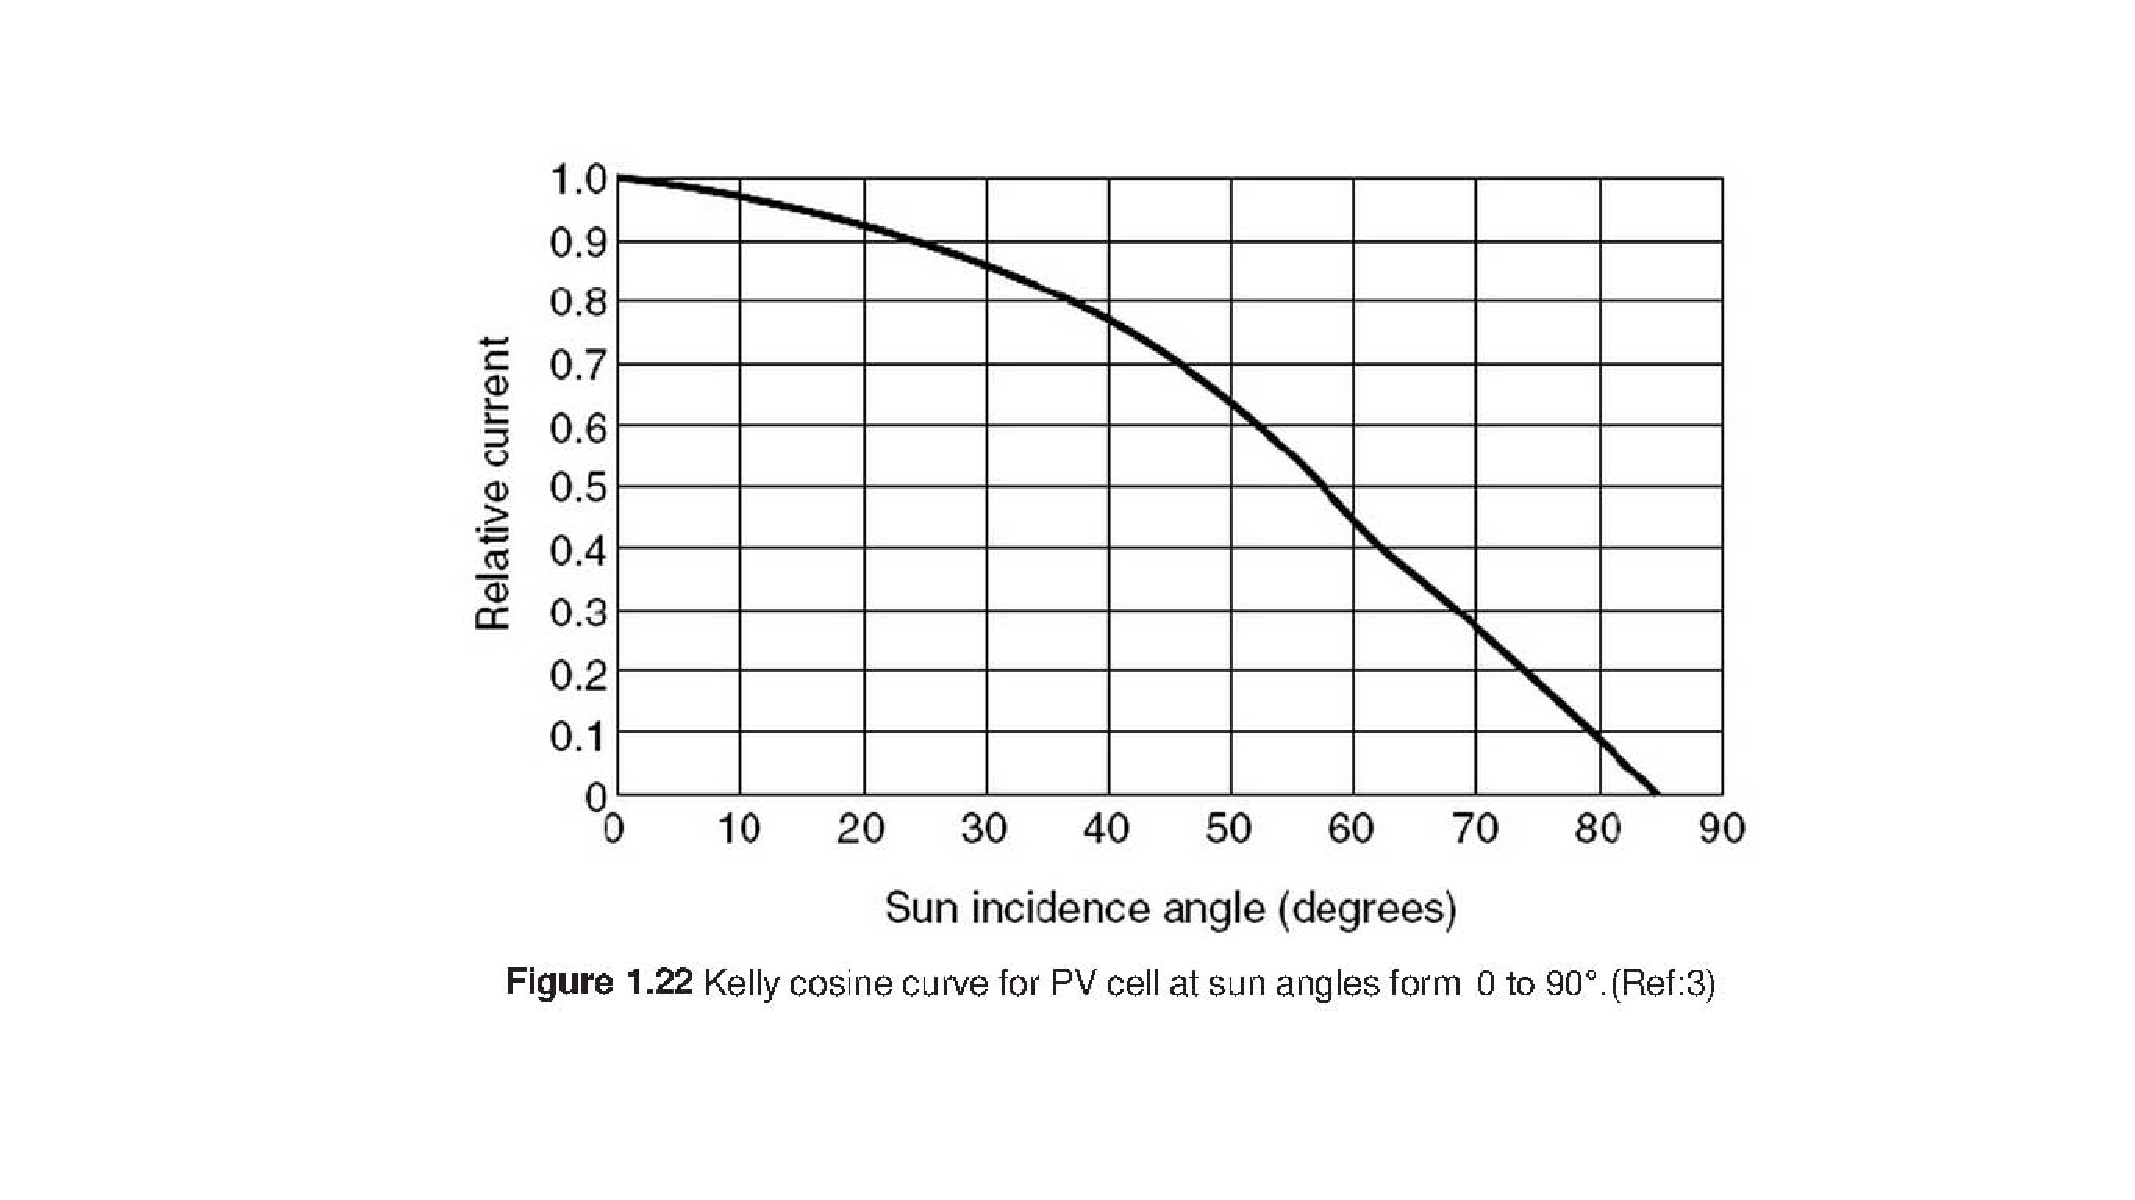
\includegraphics[scale=0.4]{figures/fig_KellyCosine}
\caption{Kelly cosine function showing how solar cell photo current depends on sun incidence angle}
\label{fig:KellyCosine}
\end{figure}
%
\subsubsection*{Solar Array Shading}
Shading on the solar panels, for example caused by airship stabilizer structures or objects in the landscape, can cause a significant drop in the cell output voltage, as described in \cite[p. 165]{Mukund}. Bypass diodes can be used to partly mitigate this issue. However, since the airship is only expected to fly at altitudes above terrain and buildings the only shading possibly expected is from the airship structure hence the \ac{MSE} design must consider this restriction.
%
\subsubsection*{Battery Temperature}
One of the most temperature critical \ac{EPS} components is the battery which must stay within its safety temperature limits. In the proposed design, only temperature monitoring is offered therefore, flight is only allowed when outdoors temperatures are well within the allowed battery temperature range. Otherwise a battery heater and more sophisticated thermal design may be necessary.
%
\subsection{Expected Performance}
The expected \ac{EPS} performance values are listed in Table \ref{tab:expected_performance}.
%
\begin{table}[H]
\centering
\caption{Expected performance of the \ac{EPS}}
\label{tab:expected_performance}
\begin{minipage}{\textwidth}
\begin{tabular}{p{0.4\textwidth}p{0.15\textwidth}p{0.35\textwidth}}
\hline
\textbf{Description} & \textbf{Symbol} & \textbf{Value}\\
\hline
Power conversion efficiency(overall) & - & $80-90\%$\\
Power output(overall) & $P_{out}$ & $\sim 57-65\,W$\\
Battery capacity & $C_{bat}$ & $7.3\,Wh$\\
Mass & $W_{EPS}$ & $\sim910\,g$\\
Total cost & - & $\sim12000\,SEK$\footnote{Solar cells are significantly more expensive than anticipated. A request for more funds is under preparation.}\\
\hline
\end{tabular}\par
\vspace{-0.75\skip\footins}
\renewcommand{\footnoterule}{}
\end{minipage}
\end{table}